\chapter{Schichtenmodelle}
Quelle: DA - Daniels Teil
\subsection*{Schichtenmodel}
Das \textbf{Schichtenmodel} ist ein im Bereich der Softwarearchitektur häufig verwendetes Strukturierungsprinzip, indem Schichten immer auf die Resourcen der unteren Schicht zugreifen können, ohne sich Gedanken um deren Format oder ähnliches machen zu müssen, während sie selbst der next höheren Schicht fixierte Objekte zur Verfügung stellen. In der Netzwerktechnik gibt es zwei etablierte Schichtenmodelle.
\subsubsection{OSI}
Das \textbf{OSI-Layer Modell} wurde 1984 von der International Organization for Standardization (ISO) als Standardreferenzmodell für Telekommunikation in Netzwerken festgelegt.\\
Das OSI-Layer Modell teilt die gesamte Kommunikation in einem Netzwerk in 7 Schichten auf, welche nach oben hin immer weiter abstrahieren, wobei eine Ebene immer die Ebene über sich bedient und von der unteren Ebene bedient wird.\\
\paragraph{Layer 1 - Physical Layer}
Die erste Ebene ist auch die am wenigsten abstrahierte Ebene.\\
Wie der Name schon andeutet, geht es beim \textbf{Physical Layer} um die \textbf{physikalischen Eigenschaften} der Verbindung. Dazu gehören Pin Layout, Leitungsimpedanzen oder welche Art der Verbindung (Koaxial Kabel, Lichtwellenleiter, ..) verwendet wird. Auch die Art der verwendeten Modulation oder das Umwandeln von Daten in Spannungen wird auf diesem Layer festgelegt.\\
Hier ist noch nicht festgelegt, wie die einzelnen Bits von einem Host zum anderen finden, sondern eher wie ein Bit auf einer Leitung überhaupt dargestellt wird und wie es transportiert wird.\\

Beispielhafte Protokolle auf dieser Ebene sind:
\begin{itemize}
\item Ethernet mit seinen Varianten
\item DSL 
\item Varianten des 802.11 Wireless Standard
\item Bluetooth
\item CAN bus
\item ...
\end{itemize}
\paragraph{Layer 2 - Data Link Layer}
Der zweite Layer im OSI-Modell ist der \textbf{Data Link Layer}.\\
Er ermöglicht die \textbf{Kommunikation zwischen zwei benachbarten Netzwerkgeräten in einem Netzwerk}. Weiters kann er Mittel zur Verfügung stellen, Fehler, welche auf dem Physical Layer auftreten können, zu beheben. So tritt hier auch die erste Adresse auf, die MAC-Adresse.\\

Beispielhafte Protokolle auf dieser Ebene sind:
\begin{itemize}
\item Ethernet
\item Token Ring
\item Spanning Tree 
\item Point-to-Point PPP
\item Multiprotocol Label Switching MLPS
\item ...
\end{itemize}
\paragraph{Layer 3 - Network Layer}
Die nächsthöhere Ebene ist der \textbf{Network Layer}.\\
Während der Data Link Layer für die Kommunikation von zwei benachbarten Netzwerkgeräten zuständig ist, ist der Network Layer für die \textbf{End-to-End Verbindung} zuständig, welche auch über mehrere Netzwerkgeräte laufen kann, also auch über mehrere Netze hinweg. Damit müssen die Protokolle auf diesem Layer eine Möglichkeit zur Adressierung bereitstellen, welche auch auf große Entfernungen, im logischen Sinne, eindeutig sind. Eine Möglichkeit sind die bereits besprochenen IP-Adressen.\\

Beispielhafte Protokolle auf dieser Ebene sind:
\begin{itemize}
\item Internet Protocol IP
\item Routing Information Protocol ARP
\item Internet Control Message Protocol ICMP
\item Internet Protocol Security IPsec
\item ...
\end{itemize}

\paragraph{Layer 4 - Transport Layer}
Die Aufgabe des vierten Layers, des \textbf{Transport Layers}, ist die \textbf{Aufteilung eines Datenstromes in Segmente}. Damit ermöglicht er es, Daten, die größer sind als nur ein Paket, zu verschicken. Des weiteren ist diese Schicht für das Aufrechterhalten des Quality of Service wichtig. Besonders wichtig sind die Protokolle TCP und UDP auf dieser Schicht. Auch werden auf dieser Ebene die Ports in die Adressen mit hineingenommen.\\

Beispielhafte Protokolle auf dieser Ebene sind:
\begin{itemize}
\item Transmission Control Protocol TCP
\item User Datagramm Protocol UDP
\item AppleTalk Trasaction Protocol ATP
\item Fibre Channel Protocol FCP
\item Stream Control Transmission Protocol SCTP
\item ...
\end{itemize}

\paragraph{Layer 5 - Session Layer}
Die fünfte Schicht des OSI-Schichtenmodells ist der \textbf{Session Layer} und für das \textbf{Aufrechterhalten der einzelnen Sessions}, also die Gespräche zwischen zwei Endgeräten zuständig. Er verwendet die unter ihm liegenden Ebenen, um seine Gespräche auf die vorhandene Netzstruktur aufzubauen und hält diese dann am Leben.\\

Beispielhafte Protokolle auf dieser Ebene sind:
\begin{itemize}
\item Net-BIOS
\item AppleTalk Session Protocol ASP
\item Point-to-Point Tunneling Protocol PPTP
\item Password Authentification Protocol PAP
\item ...
\end{itemize}

\paragraph{Layer 6 - Presentation Layer}
Die \textbf{Darstellungsschicht oder Presentation Layer} wirkt als reiner Übersetzer. Sie nimmt die Daten der Anwendungsschicht und bereitet sie so auf, dass sie für untere Schichten brauchbar werden. Falls es notwendig ist, übersetzt sie auch Dateiformate in andere Codierungen. Außerdem ist diese Ebene für die Serialisierung von komplexen Datenstrukturen in einfache \glqq flache\grqq  Byteketten, wie sie zum Beispiel in XML verwendet werden, zuständig.\\

Beispielhafte Protokolle auf dieser Ebene sind:
\begin{itemize}
\item telnet
\item Lightweight Presentation Protocol LPP
\item Independent Computing Architecture ICA (verwendet in Citrix)
\item ...
\end{itemize}

\paragraph{Layer 7 - Application Layer}
Der \textbf{Application Layer oder Anwendungsschicht} stellt das Interface dar, welches schlussendlich unter der, von dem User verwendeten, Applikation liegt. Sie ist die am meisten abstrakte Schicht und damit auch dem User am nächsten. Protokolle in dieser Schicht kümmern sich ausschließlich um die Aufgabe, welches jedes einzelne ganz speziell hat.\\

Beispielhafte Protokolle auf dieser Ebene sind:
\begin{itemize}
\item Hypertext Transfer Protocol HTTP
\item Simple Mail Transfer Protocol SMTP
\item Simple Network Management Protocol SNMP
\item Network Time Protocol NTP
\item Lightweight Directory Access Protocol LDAP
\item ...
\end{itemize}
\subsubsection{TCP/IP}
Das \textbf{TCP/IP Schichtenmodell} heißt eigentlich die \glqq \textbf{Internetprotokollfamilie}\grqq  oder \glqq \textbf{Internet Protocol Suite}\grqq . Seinen umgangssprachlichen Namen hat es von den beiden Protokollen TCP und IP, die beiden wichtigsten Protokolle des Internets, welche auch als erste in die Sammlung an Protokollen aufgenommen wurden. Doch eigentlich umfasst die Internet Protocol Suite über \textbf{500 verschiedene Protokolle}.\\
Die Internet Protocol Suite wurde von dem amerikanischen Department of Defense (DOD) entwickelt.\\


Die Internet Protocol Suite bestimmt das TCP/IP-Referenzmodel, welches ebenso wie das OSI-Schichtenmodel auf mehrere Schichten aufbaut.\\
Während das OSI-Layer Modell 7 Schichten bestimmt, verwendet das TCP/IP-Referenzmodell nur 4 Schichten. Diese wären:\\

\paragraph{Layer 1 - Link Layer}
Der Link Layer im Referenzmodell vereinigt die OSI-Schichten 1 und 2 in sich. Er ist also sowohl für die physikalischen Eigenschaften des Netzes zuständig als auch für die grundlegende Übermittlung von Daten.

\paragraph{Layer 2 - Internet Layer}
Die zweite Schicht entspricht dem Network-Layer im OSI-Schichtenmodell. Bis auf die Namensänderung gibt es jedoch keinen Unterschied, wichtigstes Protokoll ist auch hier das namensgebende Internet Protokoll.

\paragraph{Layer 3 - Transport Layer}
Der Transport Layer im TCP/IP Modell entspricht seinem gleichnamigen Bruder im OSI-Modell. 

\paragraph{Layer 4 - Application Layer}
Alle Schichten, die danach folgen würden, werden im TCP/IP-Modell zusammengefasst zum Application Layer.\\

Nun ist relativ ersichtlich, dass sich das TCP/IP-Referenzmodell sehr stark auf den Internet und den Transport Layer konzentriert, während die Layer darunter und darüber eher beinahe vernachlässigt werden. Dies ist auch der größte Kritikpunkt an diesem Modell.\\
In der Praxis wird das TCP/IP-Modell verwendet, solange die Abstrahierung nicht zu weit geht. Sollte man jedoch genauer arbeiten wird meistens auf das genormte und genauere OSI-Schichtenmodell zurückgegriffen.\\

Gegenüberstellung OSI - TCP/IP:\\
\begin{center}
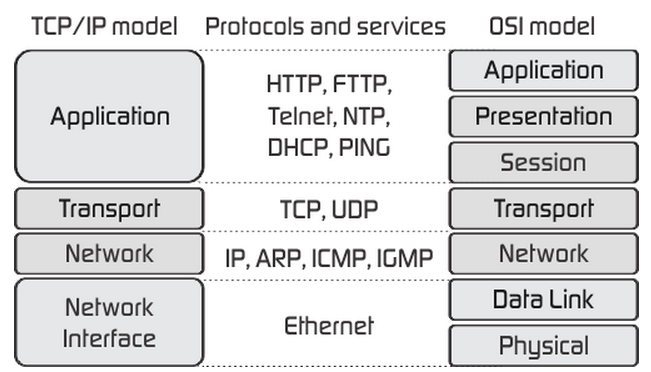
\includegraphics[scale=0.7]{files/img/lyaton_network_layer_overview.png}
\end{center}
